\begin{example}[Nested Loop with Related Iterator]
    \label{ex:threeNestedWhile}
    %
    %
    { \small
  \begin{figure}
  \centering
  \begin{subfigure}{.4\textwidth}
    \begin{centering}
    {\footnotesize
    $
    \begin{array}{l}
        \kw{threeNestedWhile}(k, m, N) \triangleq \\
        \clabel{ \assign{i}{0} }^{0} ; \\
            \ewhile ~ \clabel{i < k}^{1} ~ \edo ~ \\
            \qquad \Big(
             \clabel{\assign{j}{m}}^{2} ;\\
             \qquad \ewhile ~ \clabel{j > 0}^{3} ~ \edo ~ \\
             \qquad \qquad \Big(
              \clabel{\assign{j}{j-1}}^{4};
              \clabel{\assign{w}{i}}^{5};\\
              \qquad \qquad \ewhile ~ \clabel{w < N}^{6} ~ \edo ~
              \Big(
                \clabel{\assign{w}{w + 1}}^{7}
                  \Big); \\
                  \qquad \qquad \clabel{\assign{i}{w}}^{8}
                  \Big); \\
                  \qquad \clabel{\assign{i}{i+1}}^{9}
              \Big)
        \end{array}
    $
    }
    \caption{}
    \end{centering}
    \end{subfigure}
  \begin{subfigure}{.5\textwidth}
    \begin{centering}
  %   \todo{abstract-cfg for two round}
  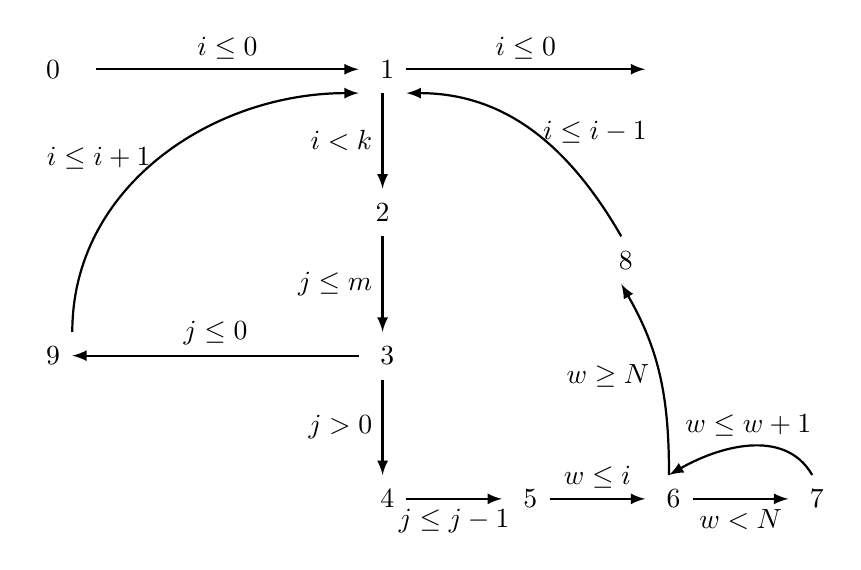
\begin{tikzpicture}[scale=\textwidth/20cm,samples=200]
  \draw[] (-7, 10) circle (0pt) node{{ $0$}};
  \draw[] (0, 10) circle (0pt) node{{ $1$}};
  \draw[] (6, 10) circle (0pt) node {{$\lex$}};
  \draw[] (0, 7) circle (0pt) node{{$2$}};
  \draw[] (0, 4) circle (0pt) node{{ $3$}};
  \draw[] (-7, 4) circle (0pt) node{{ $9$}};
  \draw[] (0, 1) circle (0pt) node{{ $4$}};
  \draw[] (3, 1) circle (0pt) node{{ $5$}};
  \draw[] (6, 1) circle (0pt) node{{ $6$}};
  \draw[] (9, 1) circle (0pt) node{{ $7$}};
  \draw[] (5, 6) circle (0pt) node{{ $8$}};
  % Counter Variables
  %
  % Control Flow Edges:
  \draw[ thick, -latex] (-6, 10)  -- node [above] {$i \leq 0$}(-0.5, 10);
  \draw[ thick, -latex] (0, 9.5)  -- node [left] {$i < k$} (0, 7.5) ;
  \draw[ thick, -latex] (0, 6.5)  -- node [left] {$j \leq m$} (0, 4.5) ;
  \draw[ thick, -latex] (0, 3.5)  -- node [left] {$j > 0$} (0, 1.5) ;
  \draw[ thick, -latex] (-0.5, 4)  -- node [above] {$j \leq 0$} (-6.5, 4) ;
  \draw[ thick, -latex] (-6.5, 4.5)  to  [out=90,in=180]  node [left] {$i \leq i + 1$ }(-0.5, 9.5);
  \draw[ thick, -latex] (0.5, 10)  -- node [above] {$i \leq 0$}  (5.5, 10);
  \draw[ thick, -latex] (0.5, 1)  -- node [below] {$j \leq j - 1$}  (2.5, 1);
  \draw[ thick, -latex] (3.5, 1)  -- node [above] {$w \leq i$}  (5.5, 1);
  \draw[ thick, -latex] (6.5, 1)  -- node [below] {$w < N$}  (8.5, 1);
  \draw[ thick, -latex] (6, 1.5)  to [out=90,in=-60] node [left] {$w \geq N$}  (5, 5.5);
  \draw[ thick, -latex] (9, 1.5)  to  [out=120,in=30] node [above] {$w \leq w + 1$}  (6, 1.5);
  \draw[ thick, -latex] (5, 6.5)  to  [out=120,in=0]  node [right] {$i \leq i - 1$ }(0.5, 9.5);
  \end{tikzpicture}
  \caption{}
    \end{centering}
    \end{subfigure}
  \caption{
  (a) The Example of Nested Loop with Related Iterator
    (b) The Abstract Execution Control Flow Graph}
      \label{fig:threeNestedWhile}
  \end{figure}
  }
\end{example}

\begin{enumerate}
    \item  \textbf{The Abstract Execution Control Flow Graph} is generated in Figure~\ref{fig:threeNestedWhile}(b).

    \item \textbf{Program Rephrase and Refinement}
    \\
    The loop free transition paths are computed as follows,
    \[
        \begin{array}{llll}
            \tpath_0 = (0 \to 1)
            &
            \tpath_1 = (1 \to 2), (2 \to 3)
            &           
            \tpath_2 = (3 \to 4), (4 \to 5), (5 \to 6)
            &
            \tpath_3 = (6 \to 7), (7 \to 6)
            \\
            \tpath_6 = (1 \to \lex)
            &
            \tpath_4 = (6 \to 8), (8 \to 3)
            &
            \tpath_5 = (3 \to 9), (9 \to 1)
        \end{array}
        \]
        \textbf{Rephrased Program}:
        \[
    \tpath_0 ; LOOP1: \rprepeat(\tpath_1; LOOP2: \rprepeat(\tpath_2; LOOP3 : \rprepeat(\tpath_3); \tpath_4); \tpath_5); \tpath_6
    \]
    \textbf{Refined Program}:
    \[
    \tpath_0 ; LOOP1: \rprepeat(\tpath_1; LOOP2: \rprepeat(\tpath_2; LOOP3 : \rprepeat(\tpath_3); \tpath_4); \tpath_5); \tpath_6
    \]
    \item \textbf{Outside-In Algorithm} : Compute Local Bound for Every program and sub programs.
    \\
$LB(\tpath_0) = 1$
\quad
$LB(LOOP2: \rprepeat(\tpath_2; \cdots)) = m $
\quad
$LB(LOOP3 : \rprepeat(\tpath_3)) = N $
\\
$LB(LOOP1: \rprepeat(\tpath_1; \cdots)) = n - N $
\item \textbf{Inside-Out Algorithm}
\begin{itemize}
    \item \textbf{Repeat Chain}
    \\
    $rp\mathcal{C}(LOOP1, \tpath_1) = \{\rprepeat(\tpath_1; \cdots)\}$ \quad
    $rp\mathcal{C}(LOOP1, \tpath_5) = \{\rprepeat(\tpath_1; \cdots)\}$ \\
    $rp\mathcal{C}(LOOP2, \tpath_2) = \{\rprepeat(\tpath_2; \cdots)\}$ \quad
    $rp\mathcal{C}(LOOP2, \tpath_4) = \{\rprepeat(\tpath_2; \cdots)\}$ \\
    $rp\mathcal{C}(LOOP3, \tpath_3) = \{\rprepeat(\tpath_3)\}$ \quad \quad
    $rp\mathcal{C}(_, \_) = \emptyset$ 
    % \\
    \item \textbf{{Local Repeat Chain Bound} for Every Transition Path $\tpath$ on its Repeat Chain}
    \\
    $rpLB(LOOP1, \tpath_1) = n - N$ \quad
    $rpLB(LOOP2, \tpath_2) = m$ \\
    $rpLB(LOOP1, \tpath_5) = n - N$ \quad
    $rpLB(LOOP2, \tpath_4) = m$ \\
    $rpLB(LOOP3, \tpath_3) = N$ \quad \quad 
    $rpLB(_, \_) = \bot $ 
    %
    \item \textbf{Loop Chain Set}
    \\
    $lp\mathcal{C}(\tpath_1) = \{LOOP1\to \tpath_1\}$ \quad
    $lp\mathcal{C}(\tpath_2) = \{LOOP1 \to LOOP2 \to \tpath_2\}$ \\
    $lp\mathcal{C}(\tpath_5) = \{LOOP1\to \tpath_5\}$ \quad
    $lp\mathcal{C}(\tpath_4) = \{LOOP1 \to LOOP2 \to \tpath_4\}$ \\
    $lp\mathcal{C}(\tpath_3) = \{LOOP1 \to LOOP2 \to LOOP3 \to \tpath_3\}$ \\
    $lp\mathcal{C}(\tpath_0) = \{\tpath_0\}$ \quad
    $lp\mathcal{C}(\tpath_6) = \{\tpath_6\}$ 
    \item \textbf{{Nested Loop Bound} for Every Transition Path $\tpath$ on its Loop Chain}
    \\
    $rpLB(LOOP1, \tpath_1) = n - N$ \\
    $rpLB(LOOP1, \tpath_5) = n - N$ \\
    $rpLB(LOOP1, \tpath_2) = n$;  $rpLB(LOOP2, \tpath_2) = m$; \\
    $rpLB(LOOP1, \tpath_4) = n$; $rpLB(LOOP2, \tpath_4) = m$ \\
    $rpLB(LOOP1, \tpath_3) = 1$; $rpLB(LOOP2, \tpath_3) = 1$; $rpLB(LOOP3, \tpath_3) = N$ \\
    $rpLB(_, \_) = \bot $ 
    \item \textbf{Path Sensitive Reachability Bound For Every Transition Path $\tpath$ }
    \\
    $psRB(\tpath_1) = n - N$ \quad
    $psRB(\tpath_2) = n \times m$ \quad
    $psRB(\tpath_0) = 1$ 
    \\
    $psRB(\tpath_5) = n - N$ \quad
    $psRB(\tpath_4) = n \times m$ \quad
    $psRB(\tpath_6) = 1$ 
    \\
    $psRB(\tpath_3) = N$ \quad
\end{itemize}
\item Step 7: Path Sensitive Reachability Bound Computation for Every Location
\\
$psRB(\{0, 1\}) = 1$ \quad
$psRB(\{2, 3\}) = n - N$ \quad
$psRB(\{4, 5, 6\}) = n \times m$ \\
$psRB(\{7, 6\}) = N$ \quad
$psRB(\{8, 3\}) = n \times m$ \quad
$psRB(\{9, 1\}) = n - N$ \\
$psRB(\{\lex\}) = 1$ 
\end{enumerate}